%!TEX program = xelatex
\documentclass[10pt]{beamer}
\usetheme[titleprogressbar]{m}

\usepackage{booktabs}
\usepackage[scale=2]{ccicons}
\usepackage{minted}

\usepackage{tikz}
\usetikzlibrary{graphs,graphs.standard}
\usetikzlibrary{arrows,positioning}
\usepackage{tkz-graph}
\usepackage{amsmath}%
\usepackage{amsthm}
\usepackage{amsfonts}%
\usepackage{amssymb}%
\usepackage{enumerate}

\usepackage{mathtools}

\DeclarePairedDelimiter\abs{\lvert}{\rvert}%
\DeclarePairedDelimiter\norm{\lVert}{\rVert}%

\makeatletter
\let\oldabs\abs
\def\abs{\@ifstar{\oldabs}{\oldabs*}}
%
\let\oldnorm\norm
\def\norm{\@ifstar{\oldnorm}{\oldnorm*}}
\makeatother


\newcommand{\leg}[2]{\left(\frac{#1}{#2}\right)}
\theoremstyle{definition}\newtheorem{proposition}{Proposition}

\usepgfplotslibrary{dateplot}

\usemintedstyle{trac}

\title{Modular Forms and Ramanujan Graphs}
\subtitle{Honours Year Project - Introductory Talk}
\date{\today}
\author{Khor Shi-Jie, supervised by Prof Gan Wee Teck}
\institute{National University of Singapore}


\begin{document}

\maketitle

\begin{frame}{Agenda}
\textbf{Modular Forms and Ramanujan Graphs}
\begin{itemize}
	\item Expander Graphs
	\item Ramanujan Graphs
	\item Construction of Ramanujan Graphs
	\begin{itemize}
	    \item Cayley Graphs
		\item Quarternion Algebra
		\item The Modular Group			
	\end{itemize}
	\item Directions of Research
\end{itemize}
\end{frame}

\section{Expander Graphs}

\begin{frame}{Graphs}
We will begin with preliminary definitions. \pause

\begin{definition}[Graph]
A graph is an ordered pair $X = (V,E)$ where $V$ is the set of vertices and $E$ is the set of edges. 
\end{definition}\pause

\begin{definition}[Path]
A path in graph $X$ is a finite sequence of vertices $v_1, v_2, \cdots, v_k$ such that $\{v_i, v_{i+1}\}$ is an edge. 
\end{definition}\pause

\begin{definition}[Connectivity]
A graph $X$ is connected if every two vertices can be joined by a path.
\end{definition}
\end{frame}

\begin{frame}{How Connected is a Graph?}
We want a notion to \textbf{measure connectivity} in a graph.\pause

In other words, we want to have a quantity to classify whether a graph is highly connected or not.

\begin{figure}
\begin{center}
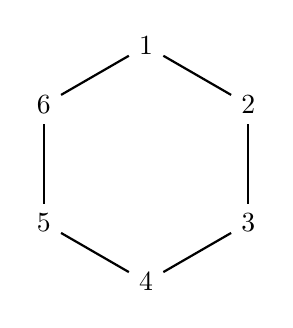
\begin{tikzpicture}[style=thick]
\graph { subgraph C_n [n=6,clockwise,radius=1.5cm] };
\end{tikzpicture}
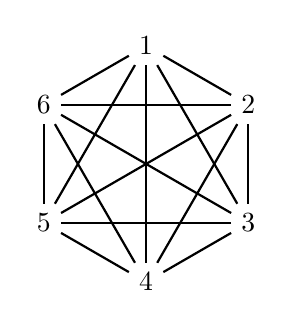
\begin{tikzpicture}[style=thick]
\graph { subgraph K_n [n=6,clockwise,radius=1.5cm] };
\end{tikzpicture}
\end{center}
\caption{Which is the more connected graph?}
\end{figure}
\end{frame}

\begin{frame}{Boundary of Vertices}
\begin{definition}[Boundary of Vertices]
Given $F \subseteq V$, define the boundary of $F$ to be the set of edges connecting from $F$ to $V - F$. We denote the set as $\partial F$. 
\end{definition}
\begin{center}
\begin{figure}
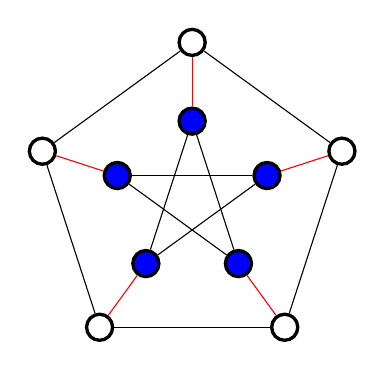
\begin{tikzpicture}[every node/.style={draw,circle,very thick}]
  \graph[nodes={draw, circle}, clockwise, radius=2cm, empty nodes] {subgraph C_n [n=5,name=A]};
  \graph[nodes={fill=blue}, clockwise, radius=1cm, empty nodes] {subgraph I_n [n=5,name=B]};

  \foreach \i in {1,2,3,4,5}{\draw[color=red] (A \i) -- (B \i);}
  \newcounter{j}
  \foreach \i in {1,2,3,4,5}{%
  	\pgfmathsetcounter{j}{ifthenelse(mod(\i+2,5),mod(\i+2,5),5)}
  	\draw (B \i) -- (B \thej);
  }
\end{tikzpicture}
\caption{Take the blue nodes as $F$, then $\partial F$ are labeled by the red edges.}
\end{figure}
\end{center}
\end{frame}

\begin{frame}{Expanding Constant}
\begin{definition}[Expanding Constant]
The expanding constant of graph $X$ is defined to be
\[h(X) := \inf \left\lbrace \frac{\partial F}{\min \{\abs{F}, \abs{V-F}\}} : F \subseteq V ,\,  0 < \abs{F} < \infty \right\rbrace\]
\end{definition}\pause

Note that if $X$ is a finite graph, we have
\[h(X) = \min\left \lbrace \frac{\partial F}{\abs{F}} : F \subseteq V,\, \abs{F} \le \frac{\abs{V}}{2}\right \rbrace\]
\end{frame}

\begin{frame}{Examples}
\vspace{-0.5cm}
The \textbf{complete graph} $K_n$ is a graph with $n$ vertices in which every vertex is connected to every other vertex. 

If $\abs{F} = l$, then $\abs{V-F} = n - l$ and hence $\abs{\partial F} = l(n-l)$. 

\begin{figure}
\begin{center}
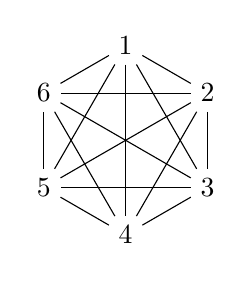
\begin{tikzpicture}
\graph { subgraph K_n [n=6,clockwise,radius=1.2cm] };
\end{tikzpicture}
\end{center}
\caption{The complete graph $K_6$.}
\end{figure}
In general, 
\[h(K_n) = n - \left\lfloor \frac{n}{2} \right\rfloor\]
\end{frame}

\begin{frame}{Examples}
\vspace{-0.5cm}
The \textbf{cycle} $C_n$ is a graph with $n$ vertices in which the entire graph is a cycle (circuit).

\begin{figure}
\begin{center}
\begin{tikzpicture}
\graph { subgraph C_n [n=6,clockwise,radius=1.2cm] };
\end{tikzpicture}
\end{center}
\caption{The cycle $C_6$.}
\end{figure}
It is obvious that
\[h(K_n) = \frac{2}{\lfloor \frac{n}{2} \rfloor}.\]
\end{frame}

\begin{frame}{$k$-Regular Graphs}
\begin{definition}
A $k$-regular graph is a graph in which the degree (i.e. number of edges incident to the vertex) of each vertex is equal to $k$.
\end{definition}
\begin{center}
\begin{figure}
\begin{tikzpicture}[style=thick]
  	\graph[nodes={draw, circle}, clockwise, radius=1.5cm, empty nodes] {subgraph C_n [n=6,name=A]};
	\foreach \i in {1,2,3}{%
  		\pgfmathsetcounter{j}{\i+3}
  		\draw (A \i) -- (A \thej);
  	}
  	\node[below, draw = none, fill = none] at (A 4.south) {$X_1$};
\end{tikzpicture}
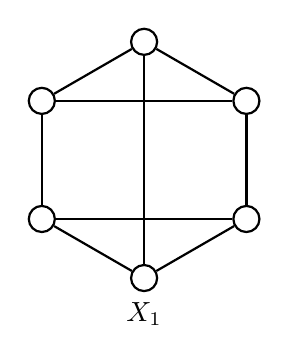
\begin{tikzpicture}[style=thick]
  	\graph[nodes={draw, circle}, clockwise, radius=1.5cm, empty nodes] {subgraph C_n [n=6,name=A]};
	\draw (A 1) -- (A 4);
	\draw (A 2) -- (A 6);
	\draw (A 5) -- (A 3);
	\node[below, draw = none, fill = none] at (A 4.south) {$X_1$};
\end{tikzpicture}
\caption{$h(X_1) = \frac{5}{3}, h(X_2) = 1$.}
\end{figure}
\end{center}
\end{frame}

\begin{frame}{Family of Expanders}
\begin{definition}
Fix a $k \in \mathbb{N}$. Let $(X_n)_{n\ge 1}$ be a sequence of finite, connected $k$-regular graphs $X_n = (V_n, E_n)$ indexed by $m \in \mathbb{N}$. $(X_n)_{n \ge 1}$ is known as a family of expanders if 
\begin{enumerate}
\item $\abs{V_n} \rightarrow +\infty$ when $n \rightarrow \infty$.
\item There exists $\epsilon > 0$ such that $h(X_n) \ge \epsilon$ for all $n \in \mathbb{N}$. 
\end{enumerate}\pause

We require each graph in the family of expanders to be $k$-regular so that the number of edges grows linearly with respect to the number of vertices.

\textbf{Question:} Is $(K_n)_{n\ge 1}$ a family of expanders? Is $(C_n)_{n\ge 1}$ a family of expanders?
\end{definition}
\end{frame}

\begin{frame}{Family of Expanders}
\textbf{Main Problem of Study:} \\
\emph{Provide explicit construction of a family of expanders.}\pause

This is an important problem, as expander graphs can be applied in 
\begin{itemize}
\item constructing good pseudorandom number generators,
\item  derandomizing a probabilistic algorithm,
\item  constructing error correcting codes, 
\item or in building probabilistically checkable proofs.
\end{itemize}
\end{frame}

\section{Ramanujan Graphs}

\begin{frame}{Adjacency Matrix}
\begin{definition}[Adjacency Matrix]
The adjacency matrix $A$ of a graph $X = (V,E)$ is a matrix indexed by the vertices of $X$ such that $A_{xy}$ is the number of edges between $x$ and $y$ in $X$. 
\end{definition}
\begin{center}
\begin{figure}
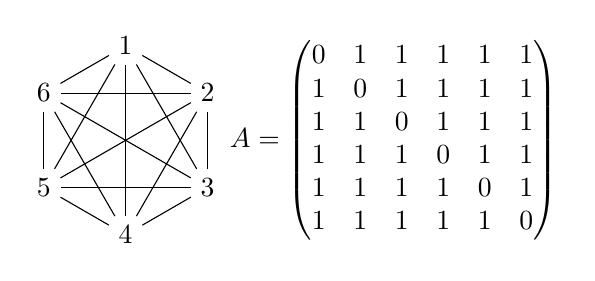
\begin{tikzpicture}
\graph { subgraph K_n [n=6,clockwise,radius=1.2cm,name=A] };
\node[right, draw = none, fill = none] at (1.2,0)  {$A = \begin{pmatrix}
0 & 1 & 1 & 1 & 1 & 1 \\
1 & 0 & 1 & 1 & 1 & 1 \\
1 & 1 & 0 & 1 & 1 & 1 \\
1 & 1 & 1 & 0 & 1 & 1 \\
1 & 1 & 1 & 1 & 0 & 1 \\
1 & 1 & 1 & 1 & 1 & 0 \\
\end{pmatrix}$};
\end{tikzpicture} 
\caption{Adjacency matrix for $K_6$.}
\end{figure}
\end{center}
\end{frame}

\begin{frame}{Eigenvalues of Graph}
Note that $A$ is a $n \times n$ symmetric matrix (where $n = \abs{V}$). \pause

Hence, $A$ has $n$ real eigenvalues. We will list the eigenvalues in decreasing order (note that the eigenvalues are listed with multiplicity):
\[k = \mu_0 \ge \mu_1 \ge \mu_2 \ge \cdots \ge \mu_{n-1}\]\pause

\begin{proposition}
Let $X$ be a finite $k$-regular graph with $n$ vertices. Then
\begin{enumerate}
\item $\mu_0 = k$;
\item $\abs{\mu_i} \le k$ for $1 \le i \le n-1$;
\item $\mu_0$ has multiplicity 1 if and only if $X$ is connected.
\end{enumerate}
\end{proposition}
\end{frame}

\begin{frame}{Examples}
The cycle $C_6$ has the following adjacency matrix
\begin{center}
\begin{figure}
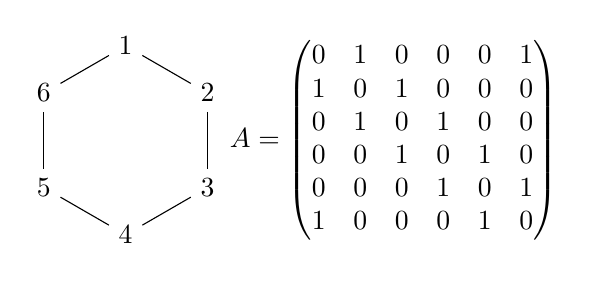
\begin{tikzpicture}
\graph { subgraph C_n [n=6,clockwise,radius=1.2cm,name=A] };
\node[right, draw = none, fill = none] at (1.2,0)  {$A = \begin{pmatrix}
0 & 1 & 0 & 0 & 0 & 1 \\
1 & 0 & 1 & 0 & 0 & 0 \\
0 & 1 & 0 & 1 & 0 & 0 \\
0 & 0 & 1 & 0 & 1 & 0 \\
0 & 0 & 0 & 1 & 0 & 1 \\
1 & 0 & 0 & 0 & 1 & 0 \\
\end{pmatrix}$};
\end{tikzpicture} 
\caption{Adjacency matrix for $K_6$.}
\end{figure}
\end{center}
The eigenvalues are $\mu_0 = 2, \mu_1 = \mu_2 = 1, \mu_3 = \mu_4 = -1, \mu_5 = -2$.
\end{frame}

\begin{frame}{Estimation of $h(X)$}
The following result bounds the expander constant of a graph $X$.
\begin{theorem}[Isoperimetric Inequality]
Let $X$ be a finite, connected, $k$-regular graph. Then
\[\frac{k - \mu_1}{2} \le h(X) \le \sqrt{2k(k-\mu_1)}\]
\end{theorem}\pause
$k - \mu_1$ is known as the\textbf{ spectral gap. }
\end{frame}

\begin{frame}{Family of Expanders}
\textbf{Rephrased Problem}

Fix a $k \in \mathbb{N}$. Find a sequence  $(X_n)_{n\ge 1}$ of finite, connected $k$-regular graphs $X_n = (V_n, E_n)$ indexed by $m \in \mathbb{N}$. $(X_n)_{n \ge 1}$ where 
\begin{enumerate}
\item $\abs{V_n} \rightarrow +\infty$ when $n \rightarrow \infty$.
\item There exists $\epsilon > 0$ such that $\boldsymbol{k - \mu_1(X_n)} \ge \epsilon$ for all $n \in \mathbb{N}$. 
\end{enumerate}

To have a good family of expanders, note that our spectral gap has to be as large as possible!
\end{frame}

\begin{frame}{Bounds on the Spectral Gap}
How large can the spectral gap be?

\begin{theorem}[Alon and Boppana]
Let $(X_n)_{n \ge 1}$ be a sequence of finite, connected, $k$-regular graphs with $\abs{V_n} \rightarrow +\infty$ as $n \rightarrow +\infty$. Then
\[\liminf_{n \rightarrow +\infty} \mu_1(X_n) \ge 2\sqrt{k-1}\]
\end{theorem}
\end{frame}
\pgfplotsset{height=7cm}
\begin{frame}{Bounds of Eigenvalues}
How can we interpret the result? (Assume $k = 5$)
\begin{figure}
\centering
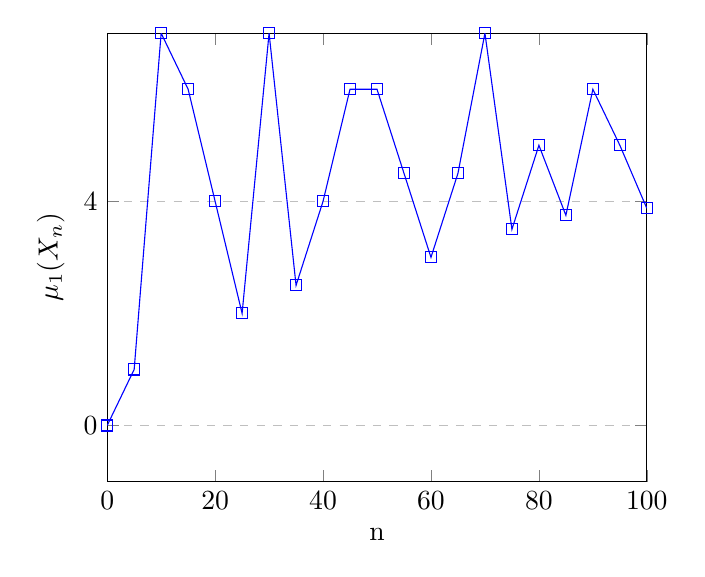
\begin{tikzpicture}
\begin{axis}[
    xlabel={n},
    ylabel={$\mu_1(X_n)$},
    xmin=0, xmax=100,
    ymin=-1, ymax=7,
    ytick={0,4},
    ymajorgrids=true,
    grid style=dashed,
]
 
\addplot[
    color=blue,
    mark=square,
    ]
    coordinates {
    (0,0) (5, 1) (10, 7) (15, 6) (20, 4) (25, 2) (30, 7) (35, 2.5) (40, 4) (45, 6) (50, 6) (55, 4.5) (60, 3) (65, 4.5) (70, 7) (75, 3.5) (80, 5) (85, 3.75) (90, 6) (95, 5) (100, 3.875)
    };
\end{axis}
\end{tikzpicture}
\end{figure}


\end{frame}

\begin{frame}{Ramanujan Graph}
\begin{definition}[Ramanujan Graph]
A finite, connected, $k$-regular graph $X$ is a Ramanujan graph if every non-trivial eigenvalue $\mu$ of $X$ satisfy $\abs{\mu} \le 2\sqrt{k-1}$. 
\end{definition}\pause

Note that a family of Ramanujan graph $(X_n)_{n \ge 1}$ in which $\abs{V_n} \rightarrow +\infty$ for $n \rightarrow +\infty$ will attain equality in Alon and Boppana's bound. \pause

Hence, a family of Ramanujan graph is \textbf{optimal from the spectral point of view.}
\end{frame}

\section{Construction of Ramanujan Graph}

\begin{frame}{The Name ``Ramanujan''}
Works of Srinivasa Ramanujan mainly centers around number theory. It is surprising to apply his result in the realm of graph theory.
\pause
Turns out that the construction of Ramanujan graphs often invoke the Ramanujan conjecture.\pause

\begin{theorem}[Ramanujan-Petersson conjecture]
Define the Ramanujan's $\tau$ function to be the Fourier coefficients of the cusp form $\Delta(z)$\footnote{We have $\Delta(z) = q - 24q^2 + 252q^3 - 1472q^4 + 4830q^5 - \cdots$ where $q = e^{2\pi iz}$.} of weight 12. Then
\[\abs{\tau(p)} \le 2p^{\frac{11}{2}}\]
\end{theorem}
\end{frame}

\begin{frame}{Cayley Graphs}
We need to find a good source of family of graphs.\pause

\begin{definition}[Cayley Graph]
Let $G$ be a group. Choose $S \subseteq G$ such that $S$ is symmetric, i.e. $S = S^{-1}$. 

The Cayley graph $\mathcal{G}(G, S)$ is defined with the following vertex set and edge set:
\begin{align*}
V &= G\\
E &= \{\{x,y\} : x, y \in G, \exists s \in S : y = xs\}
\end{align*}
\end{definition}
\end{frame}

\begin{frame}{Examples of Cayley Graphs}

\begin{columns}
    \begin{column}{0.5\textwidth}
      \centering
      \begin{figure}
		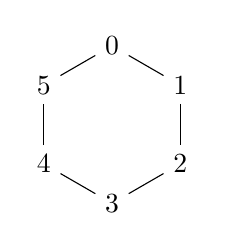
\begin{tikzpicture}
		\graph [color class=red, color class=green, math nodes, clockwise, n=6] {
		  [cycle={red}]
		  { [red]   0, 1, 2, 3, 4, 5}
		};
		\end{tikzpicture}
		\caption{$G = \mathbb{Z}_6, S = \{-1, 1\}$. }
	  \end{figure}
    \end{column}
    
    \begin{column}{0.5\textwidth}
      \centering
      \begin{figure}
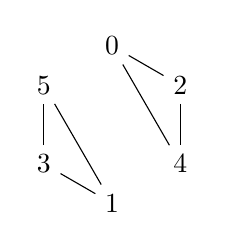
\begin{tikzpicture}
\graph [color class=red, color class=green, math nodes, clockwise, n=6] {
  [cycle={red}, cycle = {green}]
  { [red]   0, 2, 4 },
  { [green]   1, 3, 5 }
};
\end{tikzpicture}
\caption{$G = \mathbb{Z}_6, S = \{-2, 2\}$. }
\end{figure}
    \end{column}
  \end{columns}

\end{frame}

\begin{frame}{Examples of Cayley Graphs}

		
		\begin{figure}
		\centering
			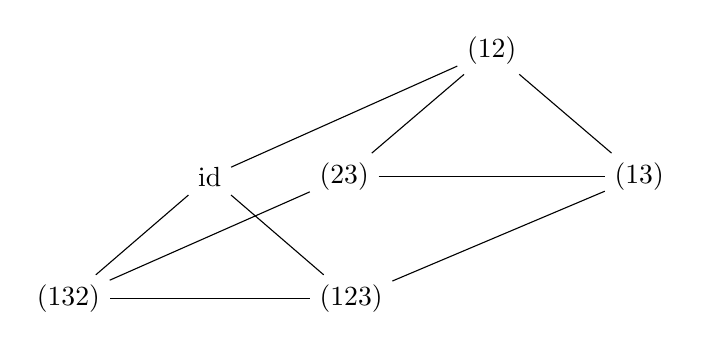
\begin{tikzpicture}
			 \node (id) at (0,0) {id};
			 \node (132) [below left=of id] {(132)};
			 \node (123) [below right=of id] {(123)};
			 \node (23) [right=of id] {(23)};
			 \node (12) [above right=of 23] {(12)};
			 \node (13) [below right=of 12] {(13)};
			 \draw (id) -- (132);
			 \draw (123) -- (132);
			 \draw (id) -- (123);
			 \draw (id) -- (12);
			 \draw (132) -- (23);
			 \draw (123) -- (13);
			 \draw (23) -- (12);
			 \draw (23) -- (13);
			 \draw (12) -- (13);
			\end{tikzpicture}
			\caption{$G = \text{Sym}_3, S = \{(123), (132), (12)\}$.}
		\end{figure}

\end{frame}

\begin{frame}{Modular Group}
What should the choice of $G$ and $S$ be to generate a family of Ramanujan graphs?
\pause
Since the Ramanujan conjecture is related to modular forms, it is no surprise that $G$ is chosen to be the  modular group.
\pause
\begin{definition}[Modular Group on Field $K$]
Suppose $K$ is a field. We define $PSL_2(K)$, the modular group on the field $K$, to be \footnote{ Denote $GL_2(K)$ as the group of invertible $2 \times 2$ matrices with entries in $K$, and $SL_2(K)$ as the subgroup of $GL_2(K)$ of matrices with determinant equals to 1. }
\[PSL_2(K) = SL_2(K) \left. \middle/ \left \lbrace \begin{pmatrix}
\epsilon & 0 \\
0 & \epsilon 
\end{pmatrix} : \epsilon = \pm 1 \right \rbrace \right. \]
\end{definition}
\end{frame}

\begin{frame}{Modular Group}
We will simply denote $PSL_2(q)$ to be the modular group over the finite field of order $q$ where $q$ is a prime.

\begin{proposition}
\begin{enumerate}
\item $\abs{PSL_2(q)} = \begin{cases}
q(q^2-1) \text{ if $q$ is even} \\
\frac{q(q^2-1)}{2} \text{ otherwise}
\end{cases}$
\item $\abs{PSL_2(K)}$ is simple for $\abs{K} \ge 4$. 
\end{enumerate}
\end{proposition}
\end{frame}

\begin{frame}{Hamilton Quarternion Algebra}
How should we choose the symmetric set for our Cayley graph?\pause

\begin{definition}[Hamilton Quarternion Algebra]
The Hamilton quarternion algebra over a ring $R$, denoted by $\mathbb{H}(R)$, is a unital, associative algebra satisfying the following properties:
\begin{enumerate}
\item $\mathbb{H}(R)$ is a free $R$-module over the symbols $1, i, j, k$. Hence, 
\[\mathbb{H}(R) = \{a_0 + a_1i + a_2j + a_3k : a_0, a_1, a_2, a_3 \in R\}\]
\item 1 is the multiplicative identity.
\item $i^2 = j^2 = k^2 = -1$.
\item $ij = -ji = k; jk = -kj = i; ki = -ik = j$. 
\end{enumerate}
\end{definition}
\end{frame}

\begin{frame}{Integer Quarternions $\mathbb{H}(\mathbb{Z})$}

Given a Hamilton quarternion algebra $\mathbb{H}(R)$, define the norm $N : \mathbb{H}(R) \rightarrow R$ by
\[N(a_0 + a_1i + a_2j + a_3k) = a_0^2 + a_1^2 + a_2^2 + a_3^2.\]

We would like to investigate the irreducible elements in $\mathbb{H}(\mathbb{Z})$.\pause

\begin{proposition}
$\delta \in \mathbb{H}(\mathbb{Z})$ is irreducible in $\mathbb{H}(\mathbb{Z})$ if and only if $N(\delta)$ is prime in $\mathbb{Z}$. 
\end{proposition}
\end{frame}

\begin{frame}{Sum of Four Squares}
Using the multiplicativity of $N$ and the previous proposition, we can easily conclude the following classical result
\begin{theorem}
Every natural number is a sum of four squares.
\end{theorem}
\pause
There is a stronger version of the above theorem proven by Jacobi.

\begin{theorem}
Let $n$ be an odd positive integer. Then the number of ways to write $n$ as a sum of four squares is $8\sum_{d \mid n} d$. 
\end{theorem}
\end{frame}

\begin{frame}{Distinguished Solutions}
Note that if $\delta \in \mathbb{H}(\mathbb{Z})$ satisfy $N(\delta) = p$ \footnote{In other words, the coefficients of $\delta$ presents a way to write $p$ as a sum of four squares}, then for each $\epsilon \in \{\pm 1, \pm i, \pm j, \pm k\}$, we have $N(\epsilon \delta) = p$. \pause

Out of these 8 quarternions, we want to choose one of them and call it a \textbf{distinguished solution}.\pause

If $p \equiv 1 \pmod{4}$, then exactly one out of the four coordinates must be odd. We will choose the solution in which the real part is odd and positive to be the distinguished solution. 

If $p \equiv 3 \pmod{4}$, then exactly one out of the four coordinate must be even, and we will make a similar choice above.
\end{frame}

\begin{frame}{Distinguished Solutions}
Suppose $p = 5$, we have the following solutions to the four square problem:
\scriptsize
\begin{columns}
\centering
\begin{column}{0.13\textwidth}
\begin{align*}
&\textbf{(1, -2, 0, 0)}\\
&(-1, 2, 0, 0)\\
&(2, 1, 0, 0)\\
&(-2, -1, 0, 0)\\
&(0, 0, 1, -2)\\
&(0, 0, -1, 2)\\
&(0, 0, 2, 1)\\
&(0, 0, -2, -1)
\end{align*}
\end{column}

\begin{column}{0.10\textwidth}
\begin{align*}
&\textbf{(1, 0, -2, 0)}\\
&(-1, 0, 2, 0)\\
&(0, 1, 0, 0)\\
&(0, -1, 0, 0)\\
&(2, 0, 1, 0)\\
&(-2, 0, -1, 0)\\
&(0, -2, 0, 1)\\
&(0, 2, 0, -1)
\end{align*}
\end{column}

\begin{column}{0.10\textwidth}
\begin{align*}
&\textbf{(1, 0, 0, -2)}\\
&(-1, 0, 0, 2)\\
&(0, 1, -2, 0)\\
&(0, -1, 2, 0)\\
&(0, 2, 1, 0)\\
&(0, -2, -1, 0)\\
&(2, 0, 0, 1)\\
&(-2, 0, 0, -1)
\end{align*}
\end{column}

\begin{column}{0.10\textwidth}
\begin{align*}
&\textbf{(1, 0, 0, 2)}\\
&(-1, 0, 0, -2)\\
&(0, 1, 2, 0)\\
&(0, -1, -2, 0)\\
&(0, -2, 1, 0)\\
&(0, 2, -1, 0)\\
&(-2, 0, 0, 1)\\
&(2, 0, 0, -1)
\end{align*}
\end{column}

\begin{column}{0.10\textwidth}
\begin{align*}
&\textbf{(1, 0, 2, 0)}\\
&(-1, 0, -2, 0)\\
&(0, 1, 0, 0)\\
&(0, -1, 0, 0)\\
&(-2, 0, 1, 0)\\
&(2, 0, -1, 0)\\
&(0, 2, 0, -1)\\
&(0, -2, 0, 1)
\end{align*}
\end{column}

\begin{column}{0.10\textwidth}
\begin{align*}
&\textbf{(1, 2, 0, 0)}\\
&(-1, -2, 0, 0)\\
&(-2, 1, 0, 0)\\
&(2, -1, 0, 0)\\
&(0, 0, 1, 2)\\
&(0, 0, -1, -2)\\
&(0, 0, -2, 1)\\
&(0, 0, 2, -1)
\end{align*}
\end{column}
\end{columns}
\normalsize
The set of distinguished solutions is denoted as $S_p$\footnote{Note that we may refer to $S_p$ as a subset in $\mathbb{H}(\mathbb{Z})$ or as an integer 4-tuple interchangeably.}.
\end{frame}

\begin{frame}{Embedding Quarternions into Matrices}
Note that our distinguished set is a subset of the quarternion, yet we stated previously that we would like to choose $PSL_2(q)$ as the base group for our Cayley Graph.
\pause
First, we consider the reduction modulo $q$,
\[\tau_q : \mathbb{H}(\mathbb{Z}) \rightarrow \mathbb{H}(\mathbb{Z}_q).\]

We would like to find a way to embed $\mathbb{H}(\mathbb{Z}_q)$ into $M_2(\mathbb{Z}_q)$. 
\end{frame}

\begin{frame}{Embedding Quarternions into Matrices}
\begin{proposition}
If $K$ is a field not of characteristic 2, suppose there exists $x,y \in K$ such that $x^2 + y^2 + 1 = 0$. Then $\mathbb{H}(K)$ is isomorphic to $M_2(K)$, the two-by-two matrices over $K$.
\end{proposition}
\pause
The isomorphism is induced by $\psi: \mathbb{H}(K) \rightarrow M_2(K)$, defined as follows
\[\psi(a_0 + a_1i + a_2j + a_3k) = \begin{pmatrix}
a_0 + a_1x + a_3y & -a_1y + a_2 + a_3x \\
-a_1y - a_2 + a_3x & a_0 - a_1x - a_3y
\end{pmatrix}\]
\end{frame}

\begin{frame}{Embedding Quarternions into Matrices}
\begin{proposition}
Let $q$ be an odd prime power. Then there exists $x,y \in \mathbb{Z}_q$ such that $x^2 + y^2 + 1= 0$. 
\end{proposition}

Hence $\mathbb{H}(\mathbb{Z}_q)$ is isomorphic to $M_2(\mathbb{Z}_q)$. We denote the isomorphism by $\psi_q$. 
\end{frame}

\begin{frame}{Embedding $S_p$ into $PSL_2(q)$}
Combining the results from the previous slides, we note that
\[(\psi_q \circ \tau_q)(S_p) \subseteq GL_2(q)\] 
Note that we omitted the proof that each element in $S_p$ is mapped to an invertible matrix.
\pause
Define $\phi$ to be the projection map from $GL_2(q)$ to $PGL_2(q)$. Then we have
\[(\phi \circ \psi_q \circ \tau_q)(S_p) \subseteq PGL_2(q)\]
We denote $S_{p,q} = (\phi \circ \psi_q \circ \tau_q)(S_p)$.
\end{frame}

\begin{frame}{The Cayley Graph $X^{p,q}$}
It can be proven that $S_{p,q} \subseteq PSL_2(q)$ if $\leg{p}{q} = 1$. 

When $\leg{p}{q} = 1$, define $X^{p,q} = \mathcal{G}(PSL_2(q), S_{p,q})$. \pause

The central theorem in the research is the following:

\begin{theorem}
$X^{p,q}$ is a non-bipartite Ramanujan graph with $\frac{q(q^2-1)}{2}$ vertices.
\end{theorem}

\end{frame}
\section{Directions of Research}

\begin{frame}{Open Problem}
The main objective is to prove that $X^{p,q}$ is a family of Ramanujan graphs. \pause

\begin{theorem}
For the following values of $k$, there exist infinite families of $k$ -regular Ramanujan graphs:

\begin{enumerate}
\item $k = p + 1$, where $p$ is an odd prime.
\item $k = 3$.
\item $k = q+1$, where $q$ is a prime power.
\end{enumerate} \pause

\textbf{Open Problem: }Is it possible to form Ramanujan graphs of arbitrary degree?
\end{theorem}
\end{frame}

\begin{frame}[allowframebreaks]
 \frametitle{References}
 \nocite{*}
        \bibliographystyle{amsalpha}
        \bibliography{biblio.bib}
\end{frame}

\plain{Thank You}

\end{document}
